\documentclass{article}
\usepackage{graphicx}
\usepackage{caption}
\usepackage{subcaption}
\usepackage{url}

\title{COP290: Moodle App}
\author{Karan Singh (2013EE10465) \\ Shantanu Kumar (2013EE10798) \\ Surag Nair (2013EE10504) }

\begin{document}
\maketitle

We have designed a user friendly moodle android app. Our app had some added features to enhance the user comfort and ease of usage.

\section{User Interface}
The UI of the app comprises of six different activities alongwith six fragments. The details of different activities are as follow:\\

\begin{itemize}
\item Login Activity : On clicking the app icon this activity is invoked where user credentials are asked.\\
%Add Image
\begin{figure}[!h]
\centering
  \begin{subfigure}{.5\textwidth}
  \centering
  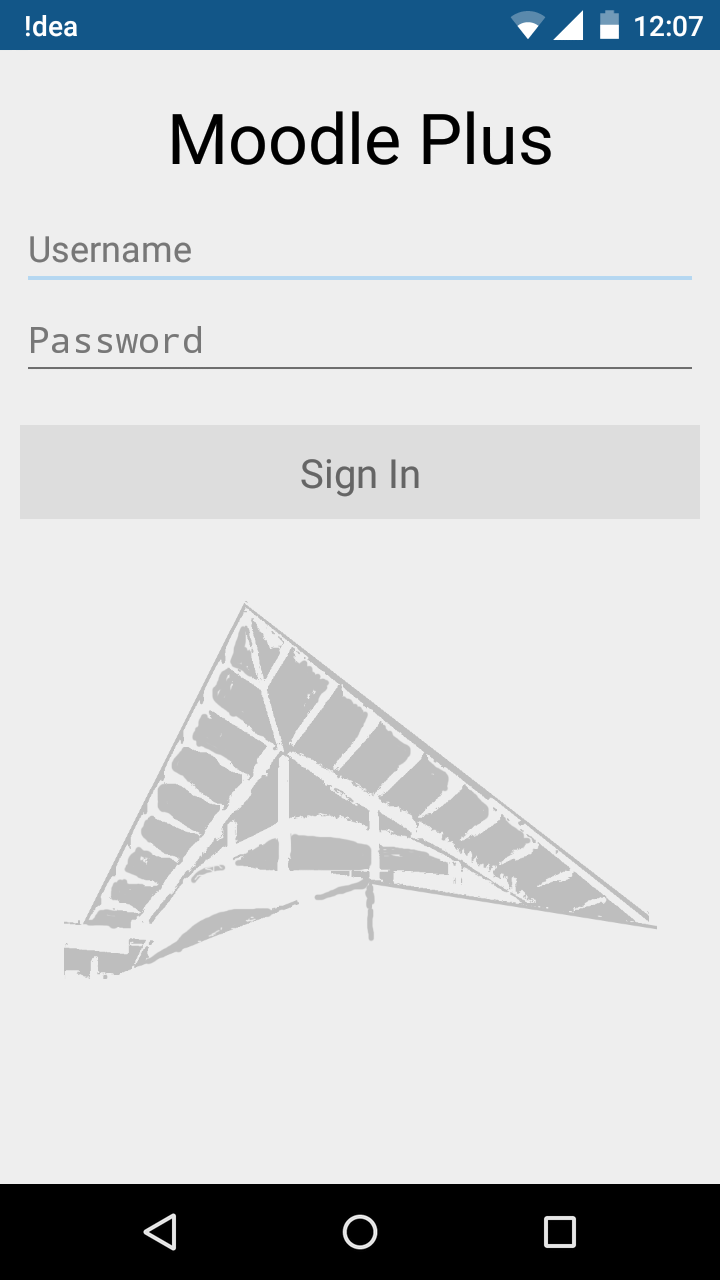
\includegraphics[width=0.8\linewidth]{pic1}
  \caption*{Sign In Screen}
  \end{subfigure}
\begin{subfigure}{.3\textwidth}
  \centering
	
\includegraphics[width=0.8\linewidth]{icon}
    \caption*{App Icon}
\end{subfigure}
\end{figure}
\item Main Activity : On successful login, this activity is called which had three fragments with different utilities. On the home page, all the registered courses of the user are listed. On the top right corner of the screen there is notifications button and on the left we have side list menu button. The side list menu has options to look at the course list, overall grades, notifications alongwith the option to sign out from the app.\\
%Add Image
\begin{figure}[!h]
\centering
\begin{subfigure}{.4\textwidth}
  \centering
	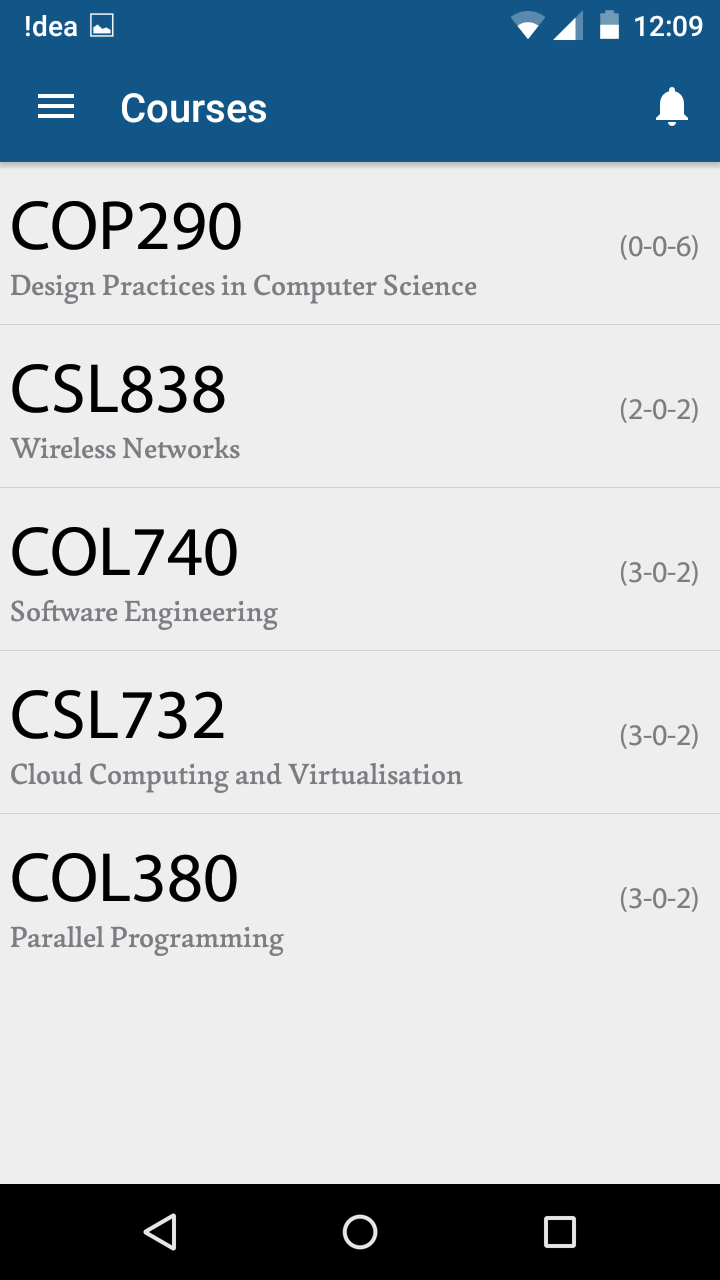
\includegraphics[width=0.8\linewidth]{pic2}
    \caption*{}
\end{subfigure}
\begin{subfigure}{.4\textwidth}
  \centering
	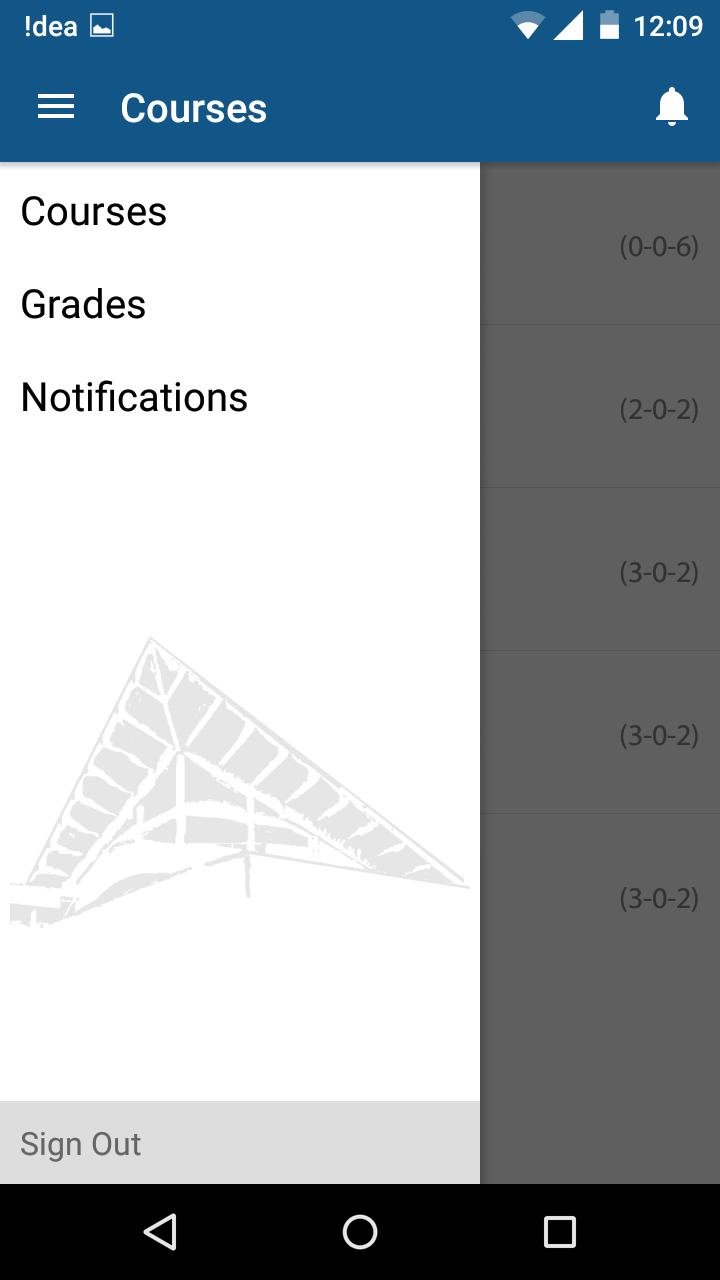
\includegraphics[width=0.8\linewidth]{pic3}
    \caption*{}
\end{subfigure}
\begin{subfigure}{.4\textwidth}
  \centering
	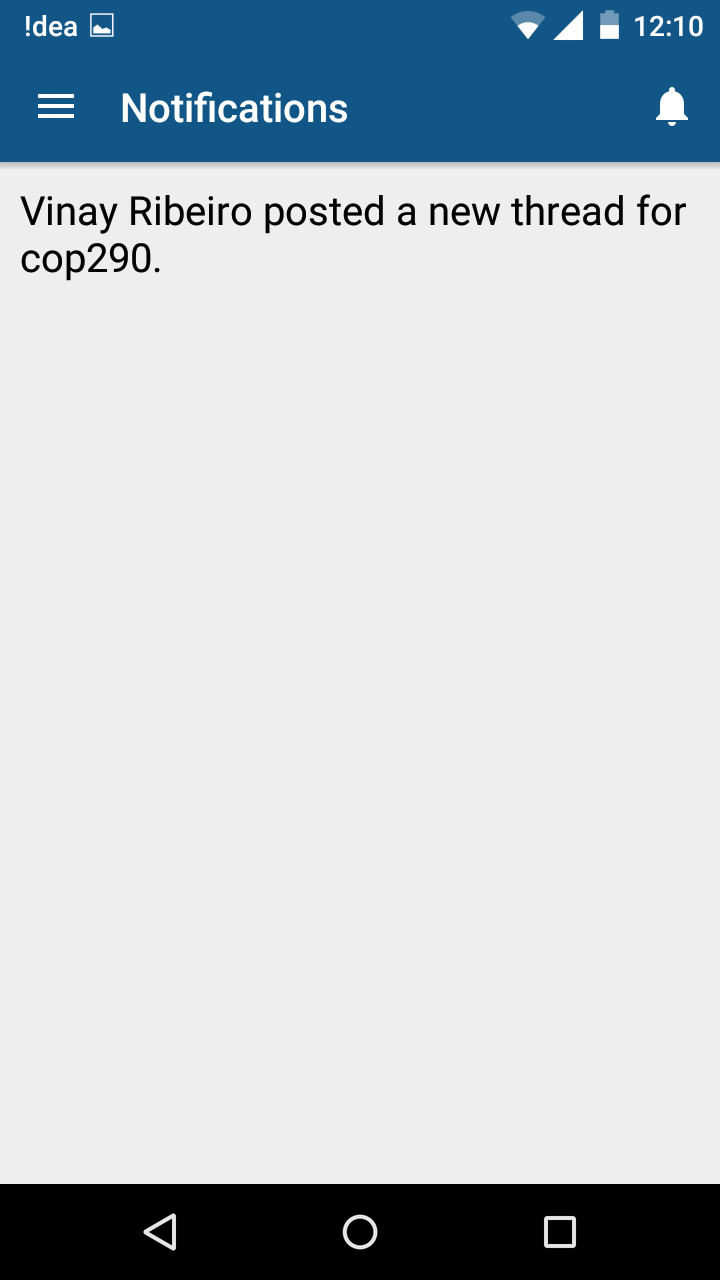
\includegraphics[width=0.8\linewidth]{pic4}
\end{subfigure}
\begin{subfigure}{.4\textwidth}
  \centering
	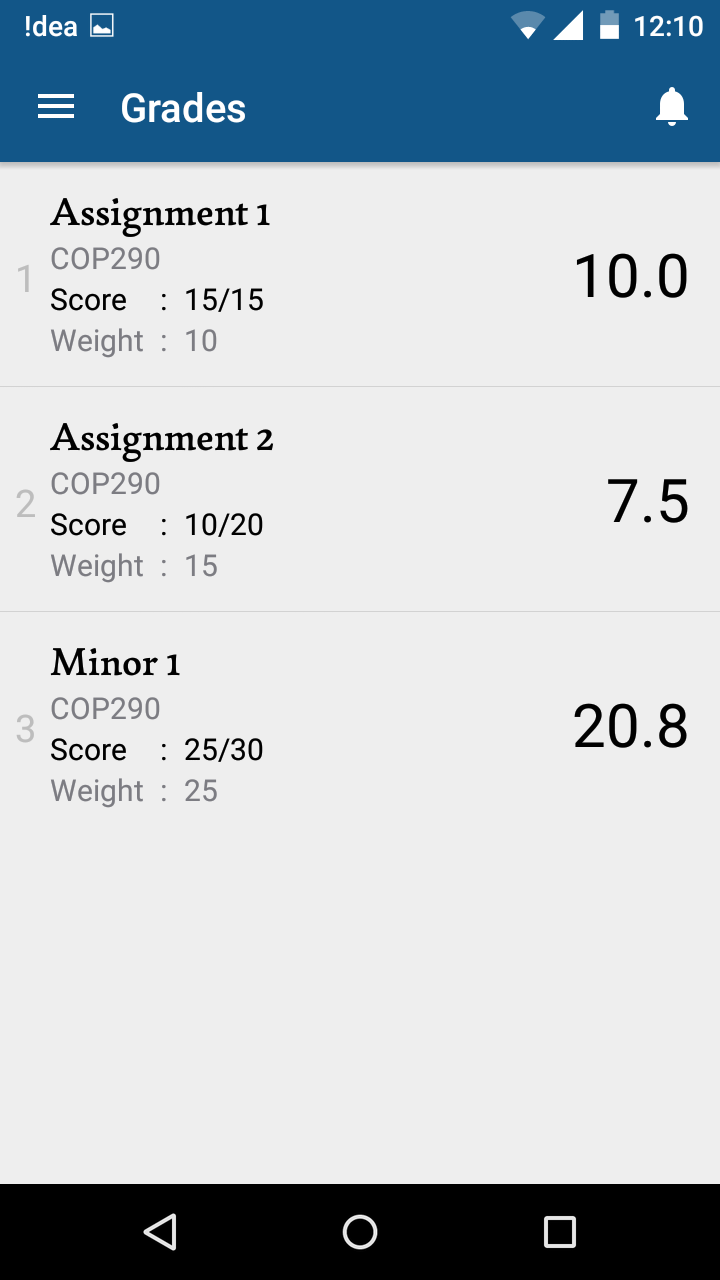
\includegraphics[width=0.8\linewidth]{pic5}
\end{subfigure}
\caption*{Main Activity Elements}
\end{figure}
\begin{itemize}
	\item Course List Fragment : This fragment displays all the registered courses of the user by populating the list from the data on the server.\\ 
%Add Image
	\item Notification Fragment : On clicking the notifications button on the top right corner of the screen this fragment is invoked enlisting all the notification pertaining to all the registered courses of the user.\\
%Add Image
	\item Grades Fragment : On clicking the grades option in the side bar list menu this fragment is invoked displaying the overall grades in different courses.\\
\end{itemize}
%Add Image
\item Course Activity : On clicking any particular course in the main activity user reaches the course activity showing various details about the selected course. This activity has three fragments corresponding to the course assignments, threads and grades.\\
\begin{figure}[!h]
\centering
\begin{subfigure}{.4\textwidth}
  \centering
	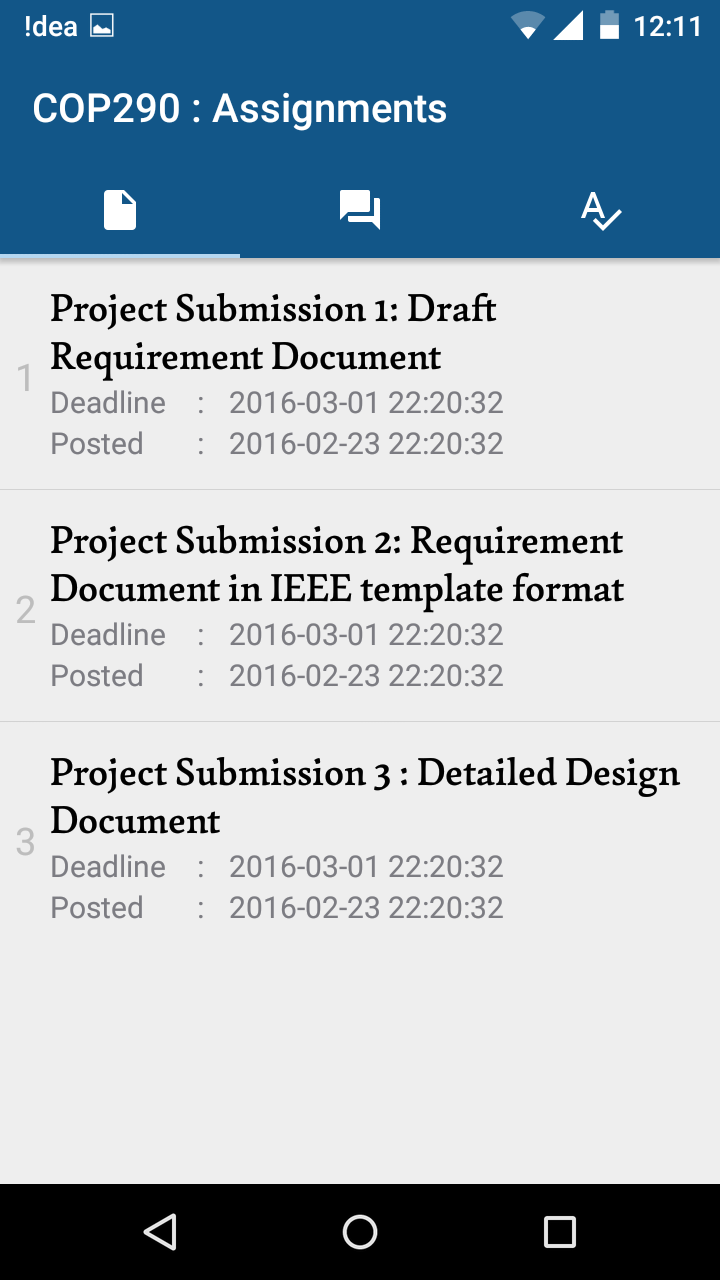
\includegraphics[width=0.8\linewidth]{pic6}
    \caption*{}
\end{subfigure}
\begin{subfigure}{.4\textwidth}
  \centering
	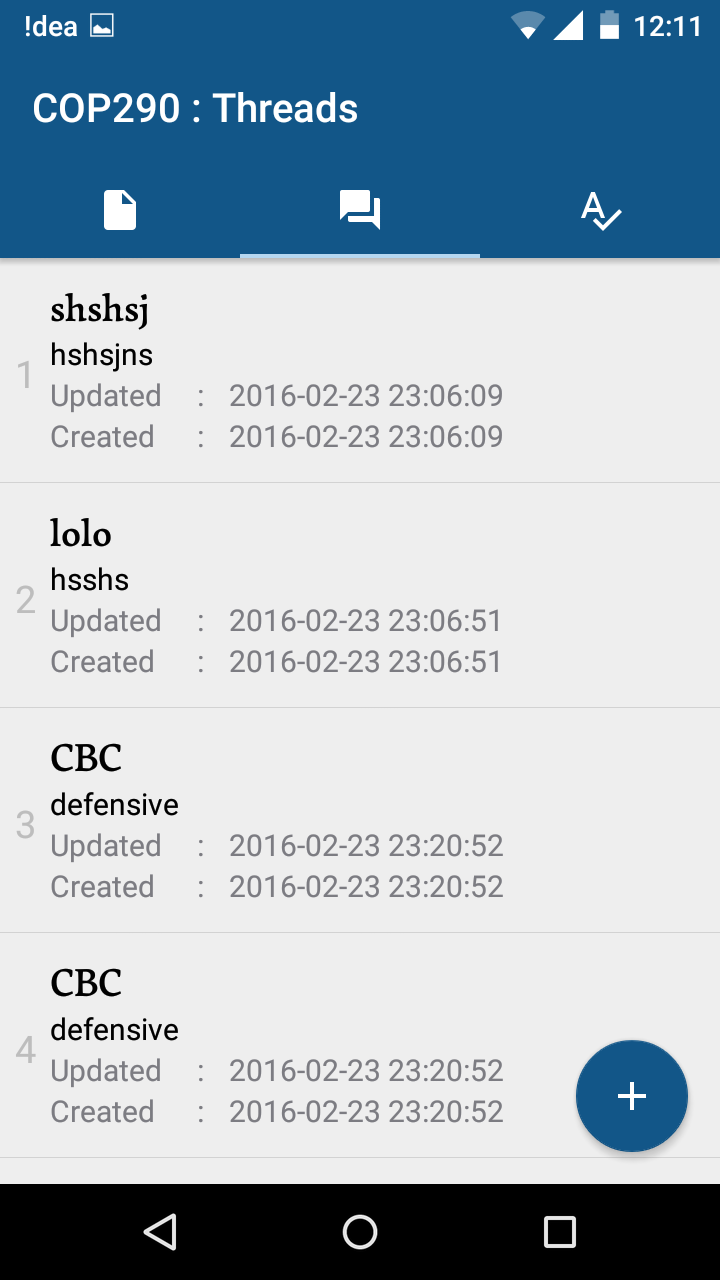
\includegraphics[width=0.8\linewidth]{pic7}
    \caption*{}
\end{subfigure}
\begin{subfigure}{.4\textwidth}
  \centering
	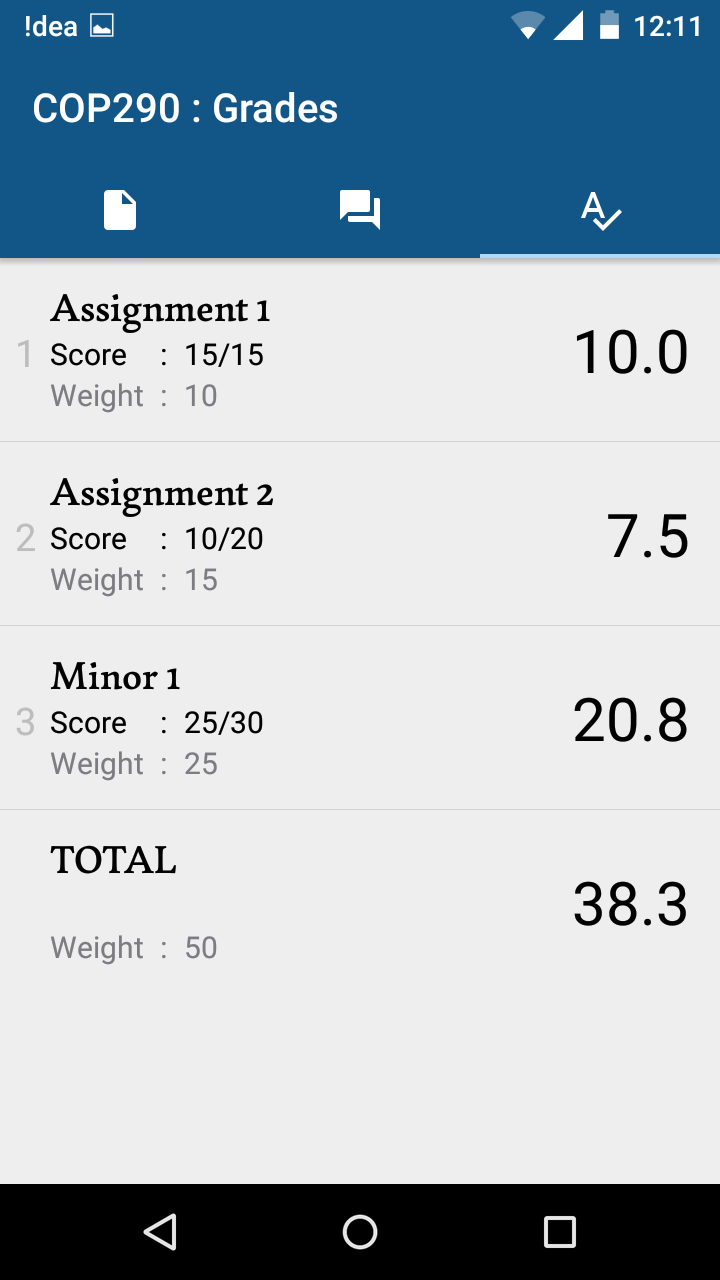
\includegraphics[width=0.8\linewidth]{pic8}
\end{subfigure}
\caption*{Course Activity Elements}
\end{figure}
	\begin{itemize}
	\item Assignments Fragment : This lists all the assignments of the particular course with limited information about each one.\\
%Add Image 
	\item Threads Fragment : All the threads pertaining to the selected course are enlisted in this fragment.\\
%Add Image
	\item Grades Fragment : List of grades secured in each assignment and exams are displayed in this fragment.\\
%Add Image
	\end{itemize}
\item Assignment Activity : On clicking a particular assignment this activity is called where complete details (date of submission, description, etc.) about that assignment are displayed.\\
%Add Image
\begin{figure}[!h]
\centering
	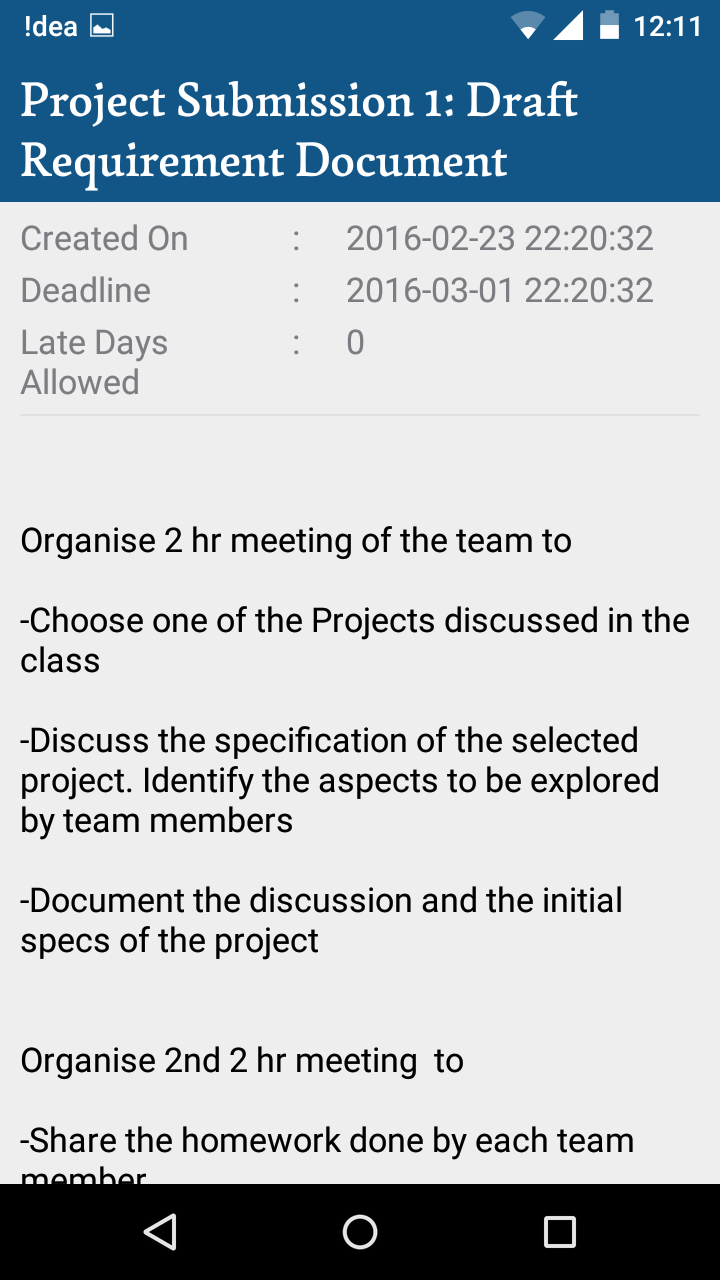
\includegraphics[width=0.35\linewidth]{pic9}
	\caption*{Assignment Activity} 
\end{figure}
\item Thread Activity : This activity has all the content of a particular thread of a particular course and is invoked when the user clicks on the list item in the course thread fragment.\\
%Add Image
\begin{figure}[!h]
\centering
\begin{subfigure}{.4\textwidth}
  \centering
	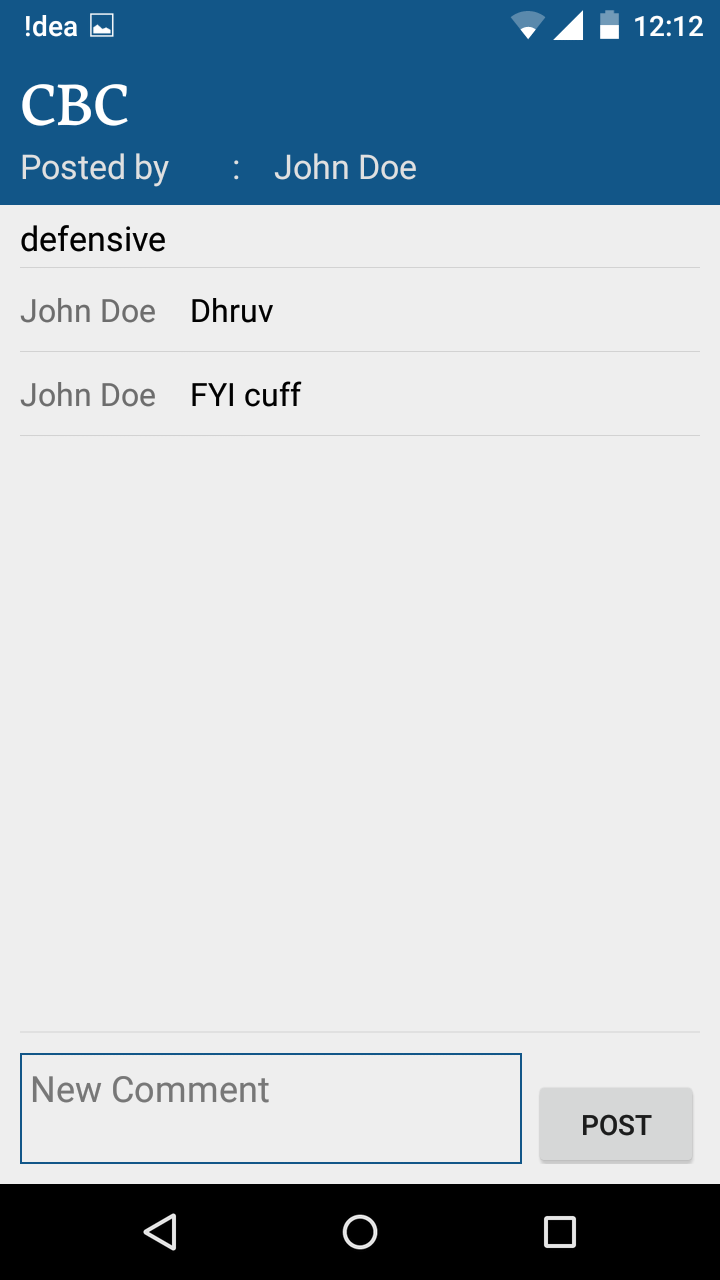
\includegraphics[width=0.8\linewidth]{pic11}
    \caption*{Thread Activity}
\end{subfigure}
\begin{subfigure}{.4\textwidth}
  \centering
	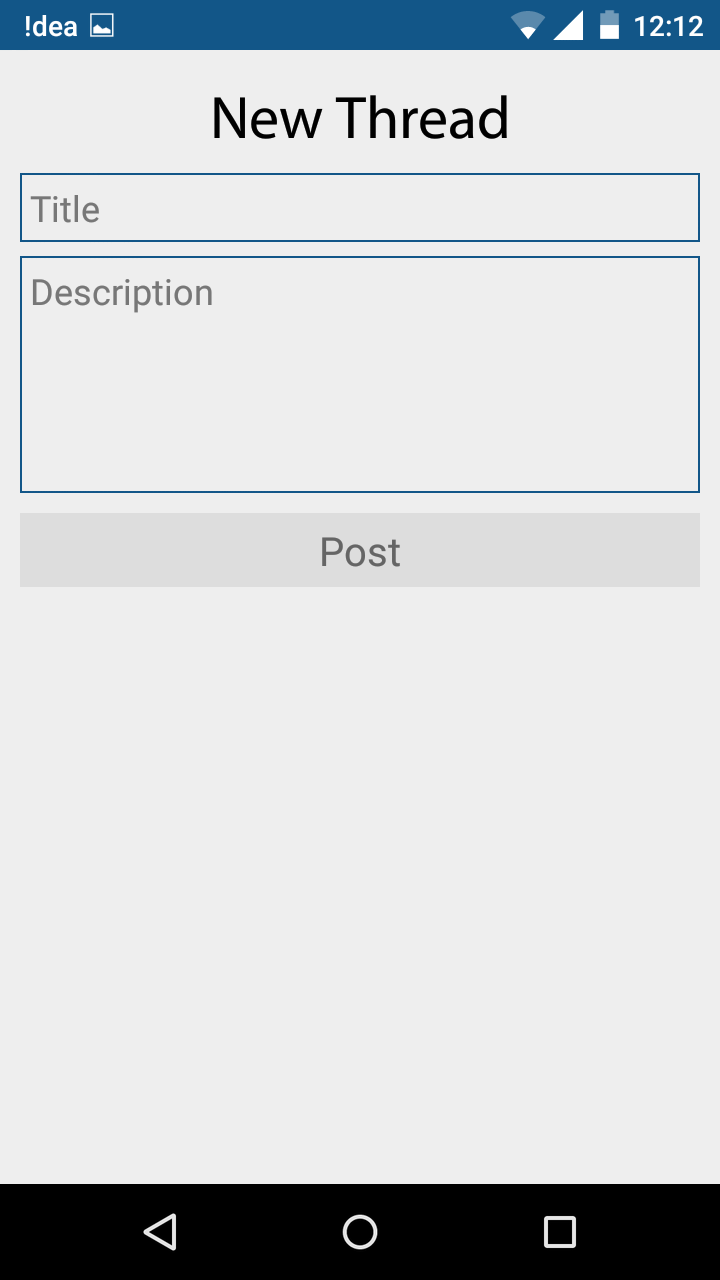
\includegraphics[width=0.8\linewidth]{pic12}
    \caption*{New Thread Activity}
\end{subfigure}
\end{figure}
\item New Thread Activity : In the course thread fragment there is button to add new thread. On pressing the button this activity is called where basic details about the thread to be created is asked.\\
%Add Image
\end{itemize}

\section{Implementation Details}

%Organization of user information (Is it in a special User class, or is it distributed in arrays for each user entry)

%(@Shantanu & Surag)Add Networking Details and the optimizations done!
\begin{itemize}
\item At the login activity the user credentials are validated by sending the request to the server and checking the response. In case of invalid login, proper message is displayed.\\
\item In order to send the request to server to fetch the particular data a common networking class is built which has functions to  returns the json response for the particular request.\\
\item In the main activity all the data regarding the registered courses, notifications and overall grades is loaded into the list-arrays. \\
\item Details about the particular course is loaded when the user clicks on the particular list. Some networking optimizations have been done to avoid the repeated server requests.\\
\item Different classes are built for effective sharing and storage of data through inheritance among various java classes to avoid repetitive code.\\
\item Periodic refresh of the threads has been incorporated so as to update the data on the app whenever there is change in data on the server.\\


%Add other features 
\end{itemize}
The project is maintained at {\em https://github.com/SourKream/ProjectWatermelon.git}.

\bibliographystyle{abbrv}
\bibliography{references}
\nocite{*}

\end{document}
